\documentclass[10pt,sigconf,letterpaper]{acmart}

\renewcommand\footnotetextcopyrightpermission[1]{} % 
%removes footnote with conference info
\setcopyright{none}
\settopmatter{printacmref=false, printccs=false, 
printfolios=false}
\pagestyle{plain}


%\documentclass[10pt,sigconf,letterpaper]{acmart}
\usepackage{color}
%\usepackage[nolist]{acronym}
%\usepackage{amsmath,amssymb}
\usepackage{pifont}
%\usepackage{enumitem}
%\usepackage{booktabs}
%\usepackage{graphicx} % embedded graphics
%\usepackage{url}
\usepackage{xcolor}
%\usepackage{times}  % Times fonts look better
%\usepackage{array}  % Extended styles for tables
%\usepackage{textcomp}

% \iffalse
\iftrue
\newcommand{\randall}{\ding{110}\ding{43}\textcolor{magenta}}
\newcommand{\pes}{\ding{110}\ding{43}\textcolor{blue}}
\newcommand{\geoff}[1]{\ding{110}\ding{43}\textcolor{violet}{#1}}
\else
\newcommand{\randall}{}
\newcommand{\pes}{}
\newcommand{\geoff}[1]{}
\fi

%\DeclareFontFamily{\encodingdefault}{\ttdefault}{\hyphenchar\font=`\-}

% \setcopyright{acmcopyright}
% \copyrightyear{2018}
% \acmYear{2018}
% \acmDOI{10.1145/1122445.1122456}

%\copyrightyear{2022}
%\acmYear{2022}
%\acmConference[IMC '22]{Internet Measurement 
%Conference}{October 25--27, 2022}{Nice, France}
\acmConference{}{}{}
%\acmBooktitle{Internet Measurement Conference (IMC '22), 
%October 25--27, 2022, Nice, France}
%\acmPrice{TBA}

\begin{document}

%\author{Submission \#19}
%\author{Audrey Randall}
%\email{aurandal@eng.ucsd.edu}
%\affiliation{UC San Diego}
%\author{Peter Snyder}
%\email{pes@brave.com}
%\affiliation{Brave Software}
%\author{Alisha Ukani}
%\email{aukani@ucsd.edu}
%\affiliation{UC San Diego}
%\author{Alex Snoeren}
%\email{snoeren@cs.ucsd.edu}
%\affiliation{UC San Diego}
%\author{Geoffrey M.\ Voelker}
%\email{voelker@cs.ucsd.edu}
%\affiliation{UC San Diego}
%\author{Stefan Savage}
%\email{savage@cs.ucsd.edu}
%\affiliation{UC San Diego}
%\author{Aaron Schulman}
%\email{schulman@cs.ucsd.edu}
%\affiliation{UC San Diego}

\title{The Challenges Associated With Decentralized Naming for Legal Takedowns}
%\renewcommand{\shortauthors}{A. Randall \textit{et al.}}

%\runningtitle{Article title}

%\subtitle{...}

%\abstract{stuff?}


\maketitle
\pagestyle{plain}

\section{Introduction}

\begin{itemize}
	\item Malware uses DNS to reach CNC servers. 
	\begin{itemize}
		\item Malware needs a naming layer because of the 
		sunk infrastructure cost: 
		any malware already deployed that uses an IP that gets blocked/taken 
		over is now useless. Malware authors want a record they can change.
		\item Naming layer needs to be hard to block at both 
		the request level and the system level, so that 
		already-distributed malware doesn't lose access and 
		become useless. 
	\end{itemize}
	\item DNS is decentralized in that there are many resolvers, but 
	centralized in that there are centralized authorities. Defenders can serve 
	legal takedown notices to those centralized authorities to block malware's 
	access to its CNC servers.
	\item Pivot: Malware is starting to use a truly decentralized naming 
	system, ``blockchain DNS.'' This creates several challenges for defenders:
	\begin{itemize}
		\item No central authority is capable of enacting domain-level takedown 
		orders
		\item For large chains, there is enough legitimate content that 
		blocking access to the whole chain is infeasible
		\item Transactions on large chains cost a lot of money. This limits 
		defenders' abilities to stage interventions like pre-registering all 
		domains listed in a malware's DGA.
	\end{itemize}
	\item We study the ecosystem and point out several places where 
	interventions are still possible, and discuss the challenges to defenders 
	and occasional advantages they gain when malware uses decentralized naming 
	such as blockchain DNS.
\end{itemize}

\section{Background}


Malware has to avoid the “sunk cost” problem, where malware that has 
already been deployed can’t be changed. This is why they don’t hard-code 
the IP of the CNC server in the deployed malware. (Actually, I think it’s 
why they need CnC servers at all.) Miscreants need to provide a layer of 
indirection --- a naming layer --- so that deployed malware can have a 
fixed, hard-coded destination to reach out to to get further instructions. 
That naming layer should be resilient to takedown efforts.

\subsection{What systems are well-suited for storing CNC names?}

From a malware author's perspective, an ideal system for recording CNC 
addresses is uncensorable at both the request level and the system level. To be 
uncensorable at the request level, there should be no central authority that 
has the ability to enforce a legal takedown notice for an individual record. To 
be uncensorable at the system level, the system should be valuable enough to 
licit actors that authorities cannot block access to it entirely without 
causing significant collateral damage to benign users.

To some extent, a trade-off exists between these features. On 
one side of the 
spectrum, protocols like Tor provide high resistance to request-level 
censorship, but they stand out, allowing systems like IDSes to detect the 
malware's presence.
%but do not have enough licit traffic to prevent authorities from 
%blocking access to the system entirely. \randall{Cite that paper that   
%said when you take away the malware, what's left is 80\% CSAM, and find other 
%citations that say defenders block Tor.}
On the other side of 
the scale, malware has repurposed ubiquitous, benign systems 
such as social media to store CNC locations. Defenders do not 
want to impose blanket bans on applications accessing social 
media URLs, but social media companies such as Facebook and 
Twitter have the capability, motivation, and are legally required to enforce 
legal takedown requests on individual posts. 

Traditional DNS is what malware uses now, with fast flux and DGA. It’s 
vulnerable to legal takedowns because it involves centralized 
authorities. Explain how legal takedowns work.

Blockchain-based naming systems present a potential threat 
because they can provide 
both qualities: they are difficult to censor at the request 
level as well as the system level. Blockchains are designed 
to prevent anyone from changing a record once it has been 
created, except for the record's owner. No central authority 
controls blockchain domains in the same way that registrars 
control traditional DNS names. Thus, even the companies 
selling blockchain domains do not have the capability to 
comply with a legal takedown request. Furthermore, even if a 
domain owner changes a domain record, the previous record 
will still be available on the chain: it cannot be deleted. 
Furthermore, some blockchains, such as Bitcoin and Ethereum, have recently 
skyrocketed in popularity as investors became interested in cryptocurrency as 
an asset class. Because these blockchains are no longer niche systems of 
interest only to a small group of technologically-savvy users, blocking access 
to them entirely will be impossible without angering a large number of 
legitimate users. As far as we are aware, cryptocurrencies and the blockchains 
they rely on are the first examples of strongly censorship-resistant systems 
that have gained a substantial community of legitimate users around the world.

Therefore, blockchain is likely to get used more in the future as a naming 
layer for the addresses of CNC servers. In fact, we already see some malware 
using it. However, blockchain is not as invincible as it claims. (summary of 
examples?)

In the remainder of this work, we detail the specific 
challenges posed by the blockchain DNS ecosystem to malware 
defenders, as well as the pieces of the ecosystem where 
effective interventions might be staged.

%Blockchains provide two censorship-resistant properties that 
%are desirable to malware authors. First, once a record 
%is created on the chain and sufficient blocks have been added 
%on top of it, it can only be updated by its owner. 
%Second, a client can access the entire blockchain as long as 
%it can reach a single participating node. However, blockchain 
%ecosystems still provide opportunities for defenders to stage 
%interventions against malware: most notably, when malware 
%connects to the chain for the first time. 


%the censorship-resistant properties of blockchains are only 
%guaranteed for transactions on the chain itself. 

%Blockchains typically present two challenges---usability and 
%performance---that incentivize users to introduce off-chain, 
%centralized authorities into the ecosystem. These 
%centralized 
%authorities can be legally compelled to enact takedown 
%requests. For example, most users connect to blockchains via 
%centralized proxies rather than by running their own nodes, 
%because running a node typically involves significant energy 
%and hardware resources. Additionally, many current users of 
%blockchain DNS domains store their records on chain in the 
%form of traditional DNS domains, rather than IP addresses. 
%These traditional domains are subject to the authority of 
%the 
%registrars that issued them. Some chains also present a 
%third 
%challenge: the high monetary cost of transactions, which 
%makes creating and updating records difficult for malware 
%authors and defenders alike. 


\section{Accessing records}

\begin{figure*}[t]
	\centering
	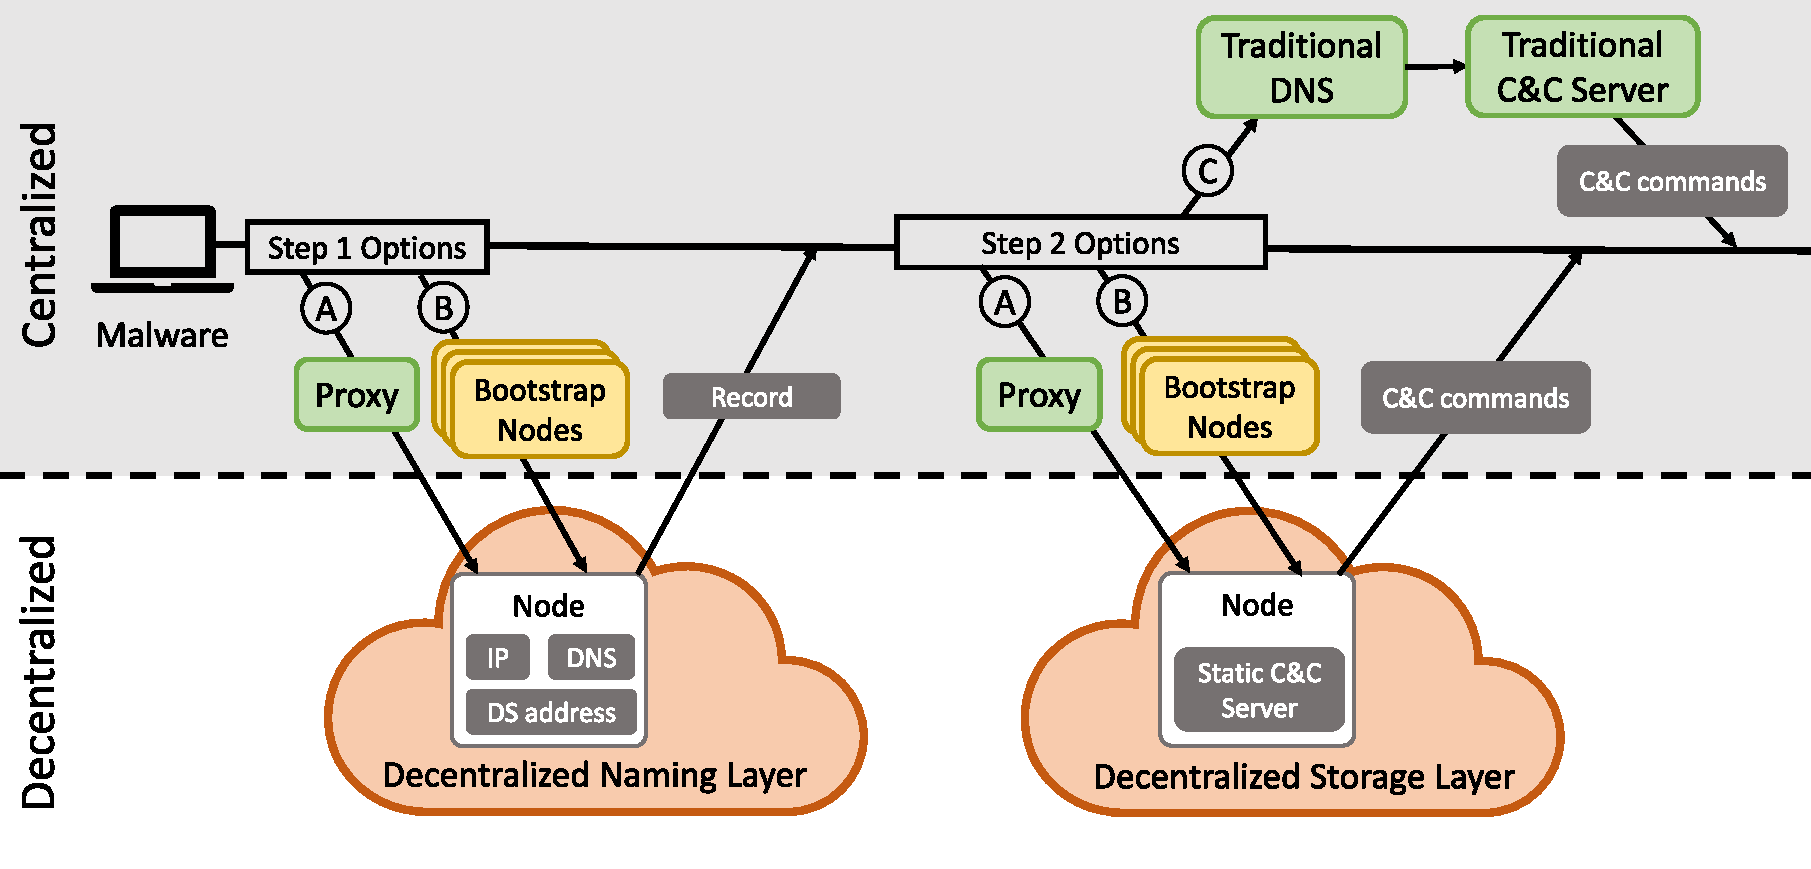
\includegraphics[width=\textwidth]{figs/malware_contacting_cnc.pdf}
	\caption{Malware must pass through centralized ``chokepoints'' to reach 
		decentralized systems, some of which might be good points for defender 
		interventions.}
	\label{fig:malware_contacting_cnc}
\end{figure*}

Given that malware requires a naming layer and it’s useful to have it on a 
blockchain, it can access it in two ways (step 1 in 
Figure~\ref{fig:malware_contacting_cnc}:
\begin{itemize}
	\item Using a proxy: These are centralized, so still good points for 
	intervention. (Insert table of proxies we've found?)
	\item Being a first class member of a chain: You find the nodes using 
	bootstrap nodes then. These are challenging for defenders to take down bc 
	of collateral damage, but can be blocklisted by IDS, 
	enterprises, antivirus. 
\end{itemize}

Anything in this figure in green is centralized enough to 
have to respond to a takedown request. Anything in yellow is 
more difficult because taking it down would have collateral 
damage, and in orange it's probably impossible to take down 
because it's truly distributed and very resilient to 
takedowns.

The record stored in the naming layer can take 
several forms. The three that we saw were IP addresses, 
traditional domains, and links to distributed file storage 
systems like IPFS and SkyNet. It's theoretically possible 
that malware could store other types of records, like links 
to social media posts, too. All of these record types except 
for the DS addresses are subject to all of the usual 
interventions. Additionally, because all blockchain records 
are public, anyone can fetch those records including 
defenders. The DS addresses are the only new thing, so we'll 
focus on those next. Also, you can only use a DS address if 
your CNC server can be implemented as a static file.

Accessing a DS system is the same as accessing a distributed 
blockchain-based naming layer: you can do it either by proxy 
or by being a first-class member of the network, in which 
case you need bootstrap nodes. Theoretically, malware can go 
straight to the storage layer, but this is unlikely to be 
feasible given the way current DS systems are set up. The 
reason malware needs 
to use a naming layer to connect to the current generation of 
distributed file storage systems is because they're 
content-addressable. As soon as the file changes, so 
does its address, and the malware that knew the old address 
is useless. 
However, this is not a fundamental limitation of distributed 
storage systems --- a system could be designed in the future 
that doesn't have this limitation.

I don't know if IPFS/SkyNet have light nodes that could be 
part of a malware payload, but there does seem to be a trend 
in that direction as chains get heavier.

\section{Modifying records}

\subsection{Name-specific chains vs. general-purpose chains}

Name-specific chains, such as Namecoin, Emercoin, and 
Handshake, tend to have fewer participants, less popularity, 
and lower transaction fees. General-purpose chains, such as 
Bitcoin and Ethereum, have naming systems built on top of the 
underlying chain, such as ENS, Unstoppable Domains, and 
Blockstack. These chains have high transaction or gas fees 
and the names are more expensive to buy (except haven't 
checked Blockstack). 

\subsection{Challenges on general-purpose chains}

\begin{itemize}
	\item High monetary cost of txns
	\begin{itemize}
		\item Defenders can't pre-register DGA domains
		\item But for malware authors, making fast flux work 
		is harder. 
	\end{itemize}
	\item Blocking malware's access to the chain
	\begin{itemize}
		\item Can't just keep every computer on the Internet 
		from accessing the chain, via IDS or whatnot, because 
		too many legit users.
	\end{itemize}
	\item \randall{Where do I put this?} Seizing control of 
	the wallet that owns a domain: 
	What about hosted wallets? If malware authors are using 
	hosted wallets to own the blockchain DNS domains, the 
	hosting service like Coinbase could presumably seize 
	them, because it has the private keys. The solution is 
	just to not use hosted wallets, but is that possible with 
	the way ENS and UD are set up? Even if it's hard, you 
	could transfer the domains to a non-hosted wallet as soon 
	as you make them. So probably not a good intervention 
	point, too easy to evade. 
\end{itemize}

\begin{figure}[t]
	\centering
	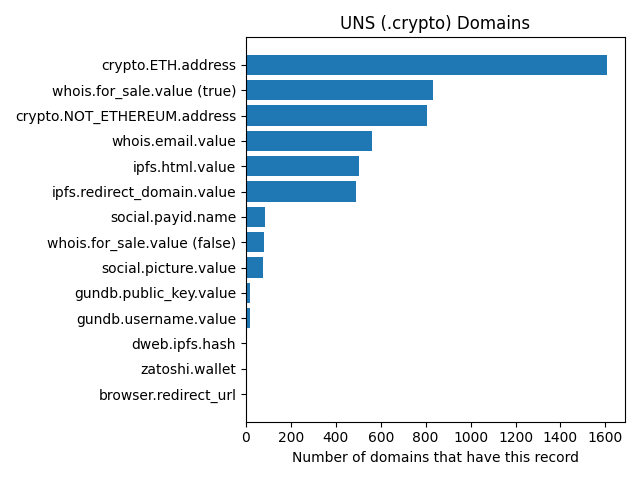
\includegraphics[width=3in]{uns_records.png}
	\caption{Types of records stored by Unstoppable 
	Domains with TLDs other than .crypto}
	\label{fig:uns_records}
\end{figure}
\begin{figure}[t]
	\centering
	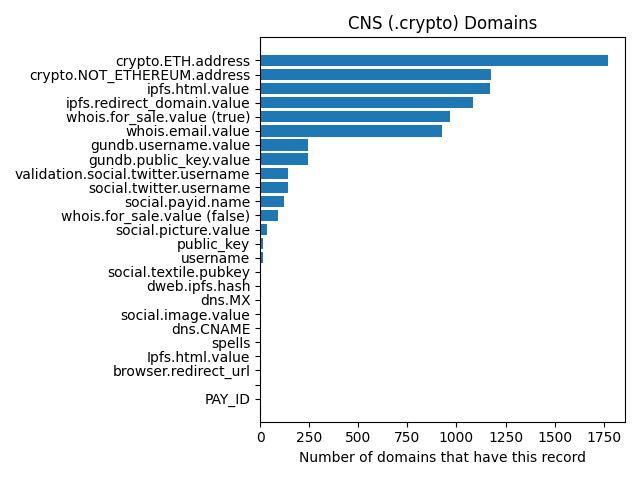
\includegraphics[width=3in]{cns_records.png}
	\caption{Types of records stored by Unstoppable Domains 
	with .crypto TLDs}
	\label{fig:cns_records}
\end{figure}


Now let's describe the specific chains in more detail. These 
systems are advertised differently - they mostly store 
wallet address records even though they're set up like DNS, 
with registrars and registries. 

\subsubsection{ENS}

Describe the registrar/registry/resolver structure.

Haven't found anything bad yet except loli-hentai.eth. This 
system, like all other uncensorable systems, will probably 
eventually attract CSAM. Describe what we did to find 
domains, how I crawled a subset.

\subsubsection{Unstoppable Domains}

Describe the registry contract and the crawled domains (I did 
crawl these didn't I?)

We don't think malware is using large chains yet because of 
the high cost of txns. If the cost goes down, or defenders 
block/take down the cheaper alternatives, malware might be 
forced to use the large chains. However, malware still seems 
to be using the small chains (Namecoin and Emercoin) a lot.

\section{Challenges on small chains}
\begin{itemize}
	\item High txn cost is less of an issue: defenders might 
	be able to register DGA domains? 
	\item Blocking the whole thing using antivirus and 
	middleboxes, or taking the whole thing down, is probably 
	possible, because there's so few legit users. Even that 
	one proxy stopped serving access to .bit domains. A 51\% 
	attack is possible on Namecoin because one pool already 
	had ~60\% of the hashing power. Also possible just to 
	blocklist every IP recorded in the chain's domain records.
\end{itemize}

The vast majority of names in ENS, Unstoppable, and Handshake 
don't have records because it's so hard to set them up, and 
while you can buy the records with no technical knowledge you 
can't assign records to them without writing code afaict. 
Also, people are mostly using these as speculative assets, 
which is another reason plenty of them have no records.

\subsection{Namecoin and Emercoin}

Plenty of DGA .bit stuff in the b-root leakage, so malware is 
still using Namecoin for sure. Should check the diffs between 
the old and new B-root dumps (numbers of hits for each TLD, 
etc)

Cite/summarize those two papers that found all sorts of 
nastiness on these chains.

\subsubsection{Handshake}

Handshake is a new blockchain-based system that aims to 
replace the root DNS 
zone. As such, it offers its users the ability to purchase 
nearly any string to 
use as a TLD. Rather than selling second-level domains 
itself, the Handshake ecosystem purports to allow its users 
to act as registrars who can sell their own domains. 
Handshake's stated goal is not to replace the traditional DNS 
system: Handshake records are designed to store the domains 
and IP addresses of traditional authoritative nameservers, 
rather than to store A, AAAA, or CNAME records. However, 
Handshake also allows users to store TXT records, which can 
contain the addresses for decentralized web hosting systems 
like Skynet or IPFS. Malware users could therefore use 
Handshake as a naming system to find content stored in 
content-addressed distributed storage systems.

``Handshake is the only naming blockchain with a lightweight 
recursive DNS resolver, which you can easily embed into 
browsers, apps, and devices.'' - 
https://learn.namebase.io/starting-from-zero/how-to-access-handshake-sites
So it can use the bootstrap nodes and participate in 
Handshake as a first class citizen, which is challenging for 
defenders.

Handshake stats:
\begin{itemize}
	\item The vast majority of names just have two GLUE4 
	records with two nameservers: “ns1.name” and “ns2.name”. 
	The IPs in these glue4 records are 44.231.6.183 and 
	54.214.136.246, respectively.
	\item Many of the most expensive TLDs (.x, .crypto, .js, 
	.8, .wallet) return an SOA record pointing to 
	``a.misconfigured.powerdns.server''
	\item ~100K had a nameserver record (all of them pointed 
	to what I assume is the Namebase resolver, except one or 
	two.) Out of those 100,000, only 101 actually had an A 
	record. 94/100 point to one IP address: 44.235.163.135. 
	That's an AWS IP that gives a 404 if you visit it with a 
	browser. Four more point to 52.43.158.89 (another AWS 
	IP), which redirects to an unconfigured distributed 
	hosting provider site. One points to 1.1.1.1, and two 
	look like someone's unconfigured personal website.
\end{itemize}

\section{What might cause a naming system to present a threat?}

What would cause a decentralized naming system to be popular enough that 
defenders wouldn't want to block access to it?
\begin{itemize}
	\item Ease of use: owners don't have to write code
	\item Affordable txns
	\item Widespread browser adoption
\end{itemize}

%\section{How big of a threat is blockchain DNS?}
%The original goal of this paper was to say whether malware 
%using blockchain to 
%contact its C\&C servers was actually a huge threat. We can 
%approach this 
%problem in two ways: (1) Map out the ecosystem and say 
%whether it's POSSIBLE, 
%(2) Check the current records being stored and say whether 
%it's already 
%happening.
%
%\section{Whether it's possible}
%
%We haven't yet started up an Ethereum light node to see if 
%it could be part of 
%a malware payload. 
%
%Stefan originally thought that because PCs/phones can't be 
%first class 
%blockchain citizens, malware won't be able to connect to a 
%blockchain without 
%using a proxy. The proxy would be an intervention point for 
%defenders to say, 
%stop serving this stuff, we have a court order. The 
%assumption there is that 
%malware can't connect to a blockchain without using a proxy. 
%I think that's 
%incorrect because the Ethereum nodes themselves use a 
%Chord-like protocol, 
%Kademlia, which I assume-but-need-to-check is a thing where 
%one node knows more 
%nodes, which know more nodes, etc. 
%
%Kademlia relies on bootstrapping, and in fact, the Ethereum 
%nodes out there 
%supposedly get their node lists from a set of bootstrap 
%nodes. You probably 
%can't outright take down the bootstrap nodes, because that 
%breaks new nodes 
%connecting to Ethereum. 
%
%Start with the simplest case - hard-coded Ethereum node 
%domains/IPs. That isn't 
%any better than just having hard coded domains/IPs of your 
%C\&C server, because 
%they're still easy for defenders to block. The caveat is, 
%maybe defenders don't 
%want to take down innocent Ethereum nodes? Because they 
%serve another, benign, 
%purpose besides malware. Stefan thinks defenders wouldn't 
%hesitate to take down 
%nodes that were hard-coded as malware access points to 
%Ethereum. But what if 
%those nodes were the official bootstrap nodes? Defenders 
%wouldn't want to take 
%those down.
%
%\subsection{Light nodes}
%
%Is it enough to just do the PING-PONG and then try to sync 
%txns? I mean, all of 
%that will be much easier if you use a light client, but 
%could you even pull 
%that code out and do it yourself? Or will the full nodes 
%say, nah we don't want 
%to connect to you? 

%Stefan was wondering which Ethereum nodes are actually used 
%for transactions, 
%and whether there's an even distribution or some nodes are 
%taking all the 
%strain. I wonder if you could say, lots of ppl are making 
%txns using Infura's 
%full nodes, let's block those txns from going out onto the 
%network? If no one 
%else can verify them, they can't get added. Or you could 
%DDoS 
%a full node to 
%prevent it sending out the message that says it's mined the 
%next block, but I'm 
%sure someone has thought of that attack already.
%
%\section{Extra interesting stuff we found along the way}
%
%\subsection{Typo squatting}


%\bibliographystyle{ACM-Reference-Format}
%\bibliography{references}
%
%\appendix
%\section{Ethics}
%
%This work raises no ethical concerns.

\end{document}
